\chapter{Evaluation}

\section{Simulation Setup}

All simulations are conducted using the gem5 Garnet cycle-accurate NoC simulator \cite{gem5} \cite{lowepower2020gem5simulatorversion200} in standalone synthetic traffic mode, without a full CPU or ISA model, to isolate network behavior. The network consists of 64 nodes arranged in an $8 \times 8$ 2D mesh topology. Each node acts as both a traffic source and destination, with packets injected according to configurable synthetic traffic patterns at a specified rate in packets per cycle per node.

The simulated clock frequency is 1 GHz. The router microarchitecture is an input-queued, virtual-channel router with credit-based flow control. Each router has a pipeline latency of 1 cycle and each link has a traversal latency of 1 cycle. The network supports three virtual networks per input port: two control virtual networks (vnets 0 and 1) and one data virtual network (vnet 2). Each virtual network contains 4 virtual channels. Control virtual channels have a buffer depth of 1 flit, while data virtual channels have a buffer depth of 4 flits. Control messages (vnets 0 and 1) consist of a single flit, whereas data messages (vnet 2) consist of 5 flits. The flit width is 128 bits (16 bytes).

The RL-based routing agent is trained over 50 million cycles, using uniform random traffic at an injection rate of 0.2 packets/cycle/node. The learned weight vectors are saved at the end of training run. The learning rate ($\alpha$), exploration rate ($\epsilon$), and discount factor ($\gamma$) are set to 0.01, 0.1, and 0.9, respectively.

For evaluation, the exploration rate is set to $\epsilon = 0$, resulting in a purely greedy policy with no further updates. Both the RL-based routing scheme and the DOR baseline are evaluated across a range of injection rates. Each configuration is simulated for 50 million cycles across multiple synthetic traffic patterns, including uniform random, neighbor, transpose, shuffle, bit reverse, and bit rotation.

The wearout state used in the RL reward is updated periodically during simulation. Link and router utilization are sampled every 1,000 cycles as a windowed average. The spatially correlated temperature map is regenerated every $10^7$ cycles. Process variation parameters ($\Delta V_{th}$, $\Delta L_{eff}$) are sampled once at initialization, ensuring identical per-router $I_{sub}$ values across both RL and DOR runs.

\section{Garnet Synthetic Traffic and Evaluation Metrics}

To evaluate the proposed routing approach under a wide range of network conditions, simulations are conducted using seven synthetic traffic patterns: uniform random, neighbor, transpose, tornado, shuffle, bit reverse, and bit rotation. These patterns generate diverse spatial load distributions, resulting in different stress profiles across routers and links and near 100\% network utilization.

Uniform random traffic selects destinations uniformly, producing a balanced load across the network. Neighbor traffic restricts communication to adjacent nodes. Transpose traffic maps each node at position $(i, j)$ to $(j, i)$. Tornado traffic sends packet from a node (i, j) in a NxM mesh to a destination node which is offset by roughly half the circumference of the mesh. Shuffle, bit reverse, and bit rotation are structured permutation patterns derived from bitwise transformations of node indices, which create asymmetric and pattern-dependent congestion across the network.

For each traffic pattern, injection rates are swept to capture both low-load and high-load regimes. For uniform random and neighbor traffic, injection rates range from 0.01 to 0.40 packets/cycle/node in increments of 0.03. For the remaining patterns, injection rates range from 0.01 to 0.20 in increments of 0.01. Each configuration is simulated for 50 million cycles.

The evaluation focuses on both performance and reliability metrics. Performance is characterized using average packet latency and throughput, while reliability is assessed using the AF derived from EM and HCI lifetime models. Together, these metrics provide a comprehensive view of the trade-offs between network efficiency and long-term wear.

\section{Results}

\subsubsection{Acceleration Factor}

To summarize the reliability improvements across traffic patterns, the mean Acceleration Factor (AF) for the weakest 10\% of components is presented using bar charts (Figures~\ref{fig:af_links_bar} and \ref{fig:af_routers_bar}). Detailed AF trends as a function of injection rate are provided in the appendix \ref{chap:app1}.

\begin{figure}[ht]
  \begin{center}
      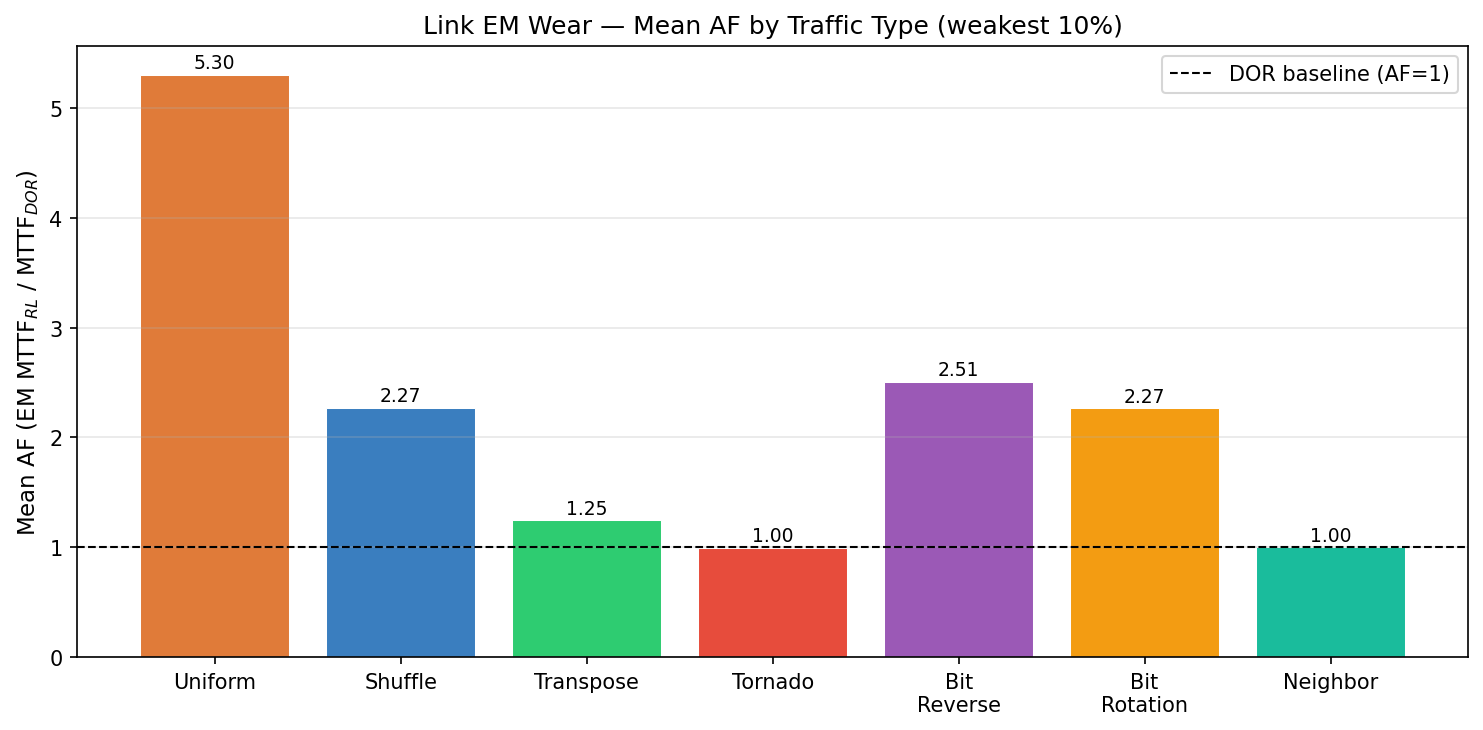
\includegraphics[width=0.95\linewidth]{body_chapters/chap_4/figs/af_weak10_bar_links.png}
      \caption[Mean EM Wear in Links]{Mean Acceleration Factor (AF) for the weakest 10\% of links under EM wear across different traffic patterns.}
      \label{fig:af_links_bar}
  \end{center}
\end{figure}

\begin{figure}[ht]
  \begin{center}
      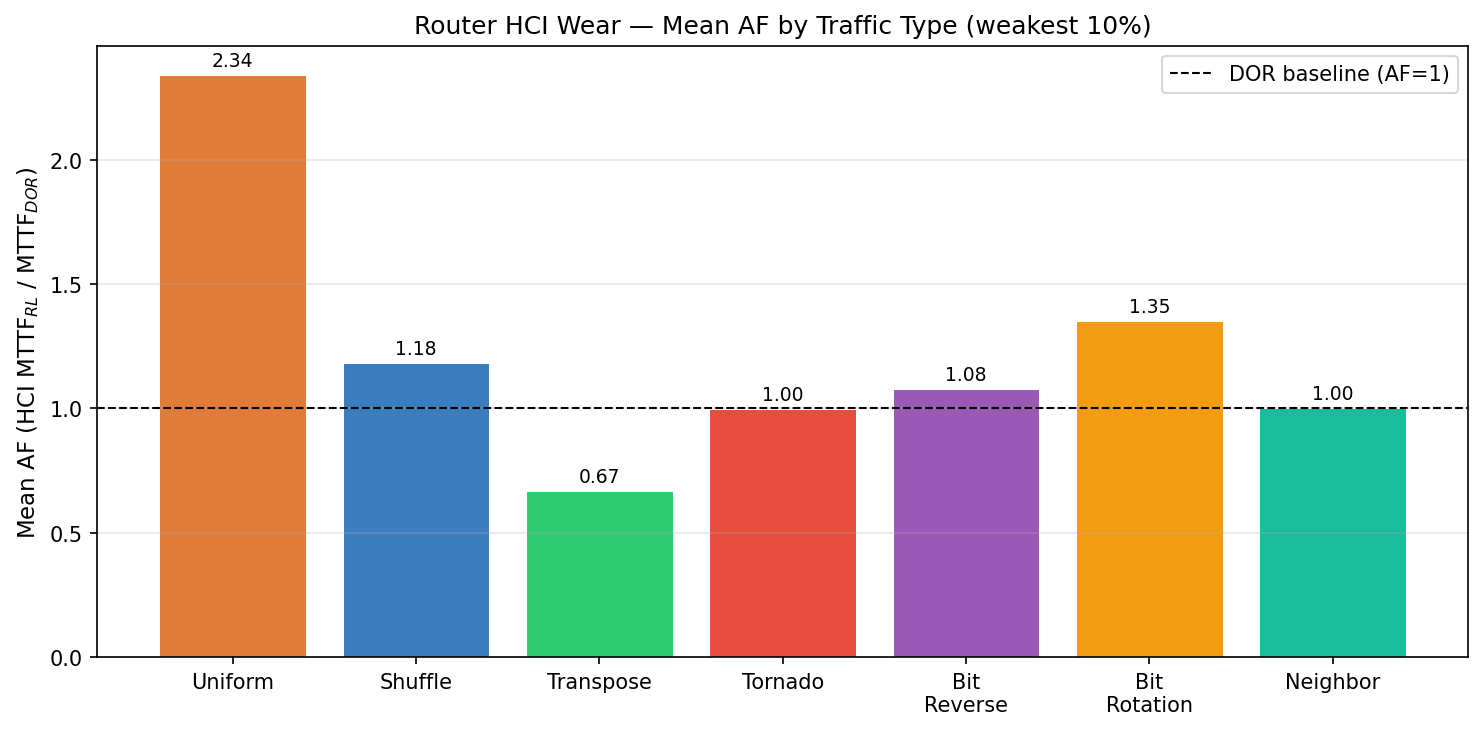
\includegraphics[width=0.95\linewidth]{body_chapters/chap_4/figs/af_weak10_bar_routers.png}
      \caption[Mean HCI Wear in Routers]{Mean Acceleration Factor (AF) for the weakest 10\% of routers under HCI wear across different traffic patterns.}
      \label{fig:af_routers_bar}
  \end{center}
\end{figure}

Overall, the proposed RL-based routing achieves significant improvements in lifetime compared to DOR, with consistently higher AF values across most traffic patterns. As expected, the improvement is more pronounced for EM than for HCI due to the quadratic dependence of EM lifetime on switching activity. Redistributing traffic away from heavily utilized links therefore yields substantial gains in EM lifetime, whereas HCI, with its linear dependence and sensitivity to process variation, exhibits more modest improvements.

For EM wear (links), the largest improvement is observed under uniform random traffic, where AF reaches approximately $5.3\times$. This reflects the ability of the RL policy to effectively balance load in a scenario with high path diversity. Shuffle and bit rotation traffic patterns yield similar improvements of approximately $2.3\times$, while bit reverse achieves around $2.5\times$. In contrast, transpose, neighbor, and tornado traffic show significantly lower gains, with AF values of approximately $1.25\times$ for transpose and close to $1.0\times$ for tornado and neighbor. This is expected, as these traffic patterns constrain packets to a limited set of shortest paths, forcing traffic through central or local links where routing flexibility is reduced.

For HCI wear (routers), a similar trend is observed, though with lower overall gains. Uniform random traffic again provides the highest improvement, with an AF of approximately $2.3\times$. Shuffle and bit rotation yield moderate improvements of around $1.2\times$. Bit reverse shows a slight improvement, while tornado and neighbor traffic exhibit little to no gain over DOR. In particular, the RL routing algorithm performs slightly worse under transpose traffic, as the routing options repeatedly stress the same set of routers along fixed shortest paths.

These results highlight two key observations. First, the effectiveness of RL-based routing is strongly dependent on the availability of path diversity. Traffic patterns that allow multiple routing choices benefit the most from adaptive routing. Second, EM benefits more than HCI due to its higher sensitivity to load redistribution, making it the dominant factor in overall lifetime improvement.

\subsubsection{Latency Analysis}

To evaluate the performance impact of the proposed routing scheme, average packet latency is measured as a function of injection rate across all traffic patterns. Representative latency curves are shown in Figures~\ref{fig:latency_curves_1}, \ref{fig:bit_rotation_latency}, \ref{fig:latency_curves_2}, \ref{fig:latency_curves_3}.

\begin{figure}[ht]
  \centering
  \begin{subfigure}{\linewidth}
    \centering
    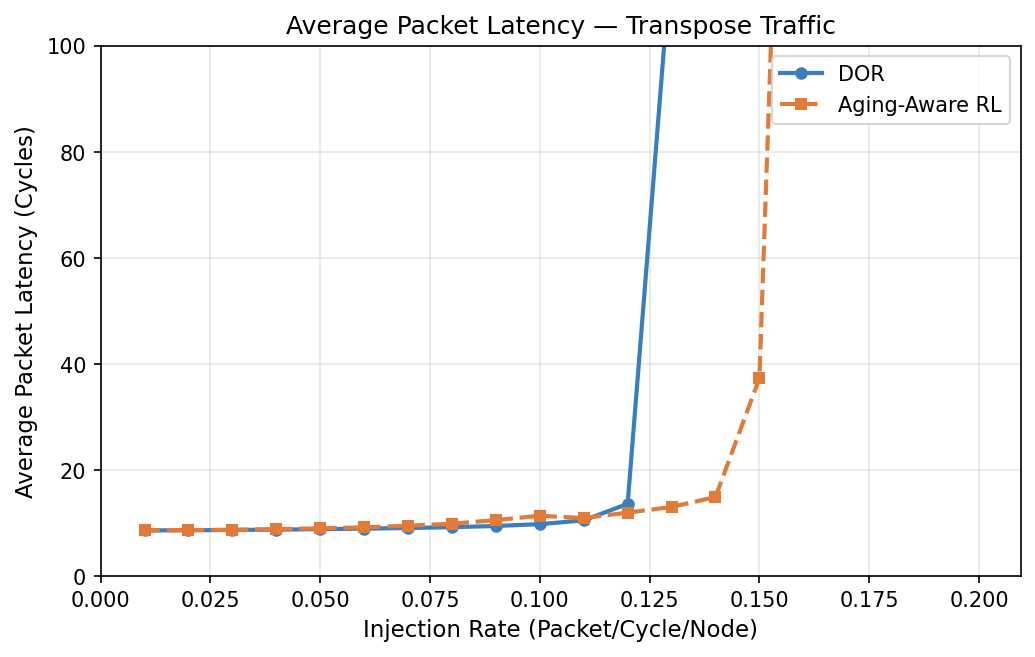
\includegraphics[width=0.8\linewidth]{body_chapters/chap_4/figs/latency_transpose.png}
    \caption{Average Packet Latency under Transpose Traffic.}
    \label{fig:transpose_latency}
  \end{subfigure}
  \vspace{1em}
  \begin{subfigure}{\linewidth}
    \centering
    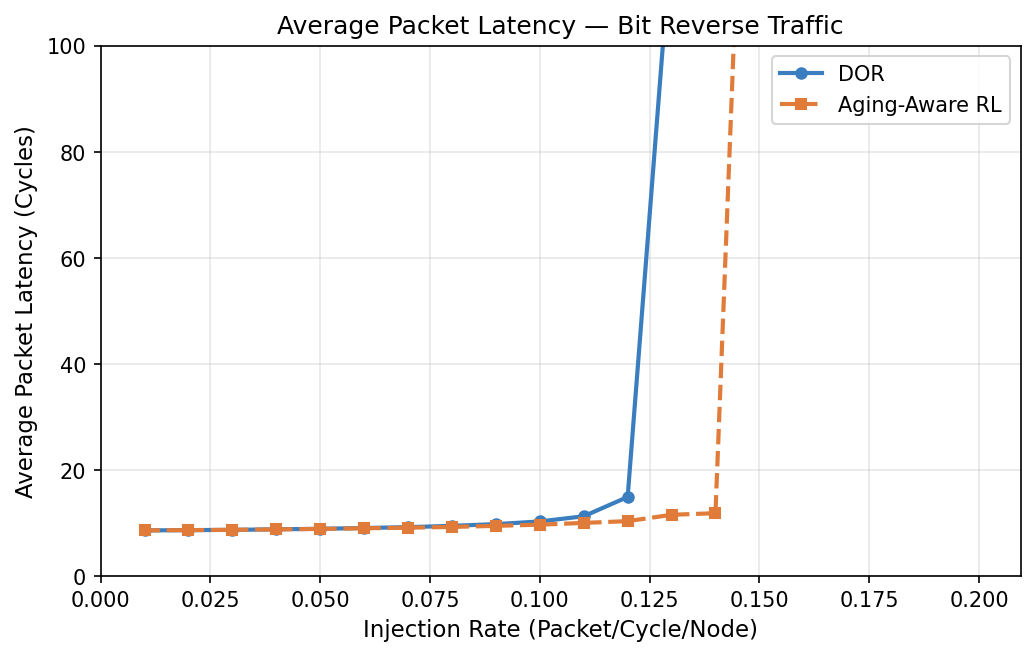
\includegraphics[width=0.8\linewidth]{body_chapters/chap_4/figs/latency_bit_reverse.png}
    \caption{Average Packet Latency under Bit Reverse Traffic.}
    \label{fig:bit_reverse_latency}
  \end{subfigure}
  \caption[Average Packet Latency (Transpose, Bit Reverse, Bit Rotation)]{Average Packet Latency vs. Injection Rate for RL-based Routing and DOR across Transpose, Bit Reverse, and Bit Rotation traffic patterns.}
  \label{fig:latency_curves_1}
\end{figure}

\begin{figure}[ht]
  \begin{center}
    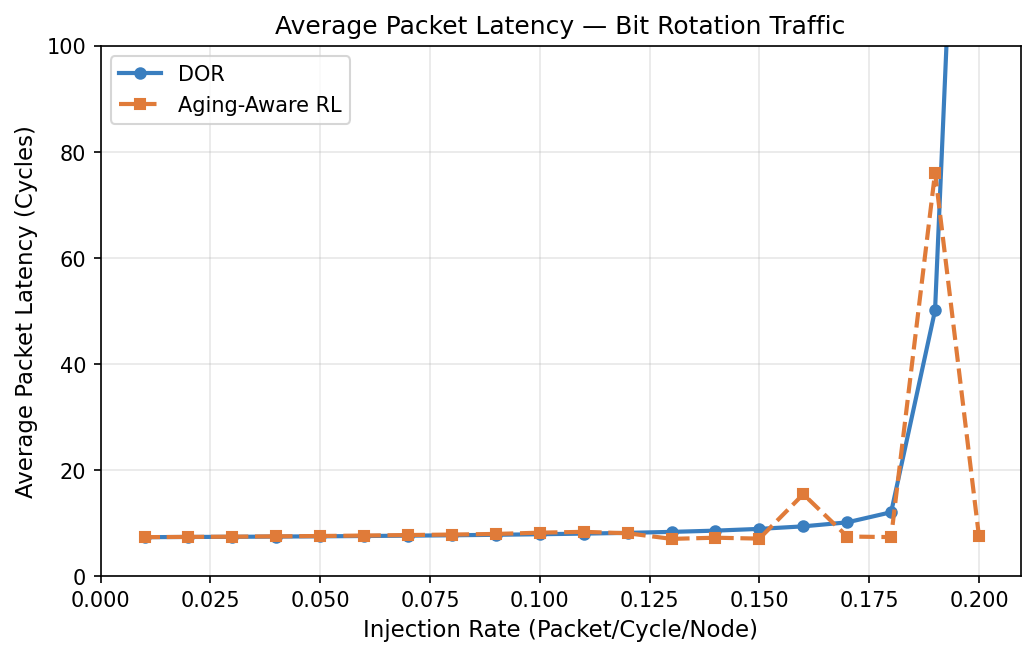
\includegraphics[width=0.8\linewidth]{body_chapters/chap_4/figs/latency_bit_rotation.png}
    \caption{Average Packet Latency under Bit Rotation Traffic.}
    \label{fig:bit_rotation_latency}
  \end{center}
\end{figure}

\begin{figure}[ht]
  \centering
  \begin{subfigure}{\linewidth}
    \centering
    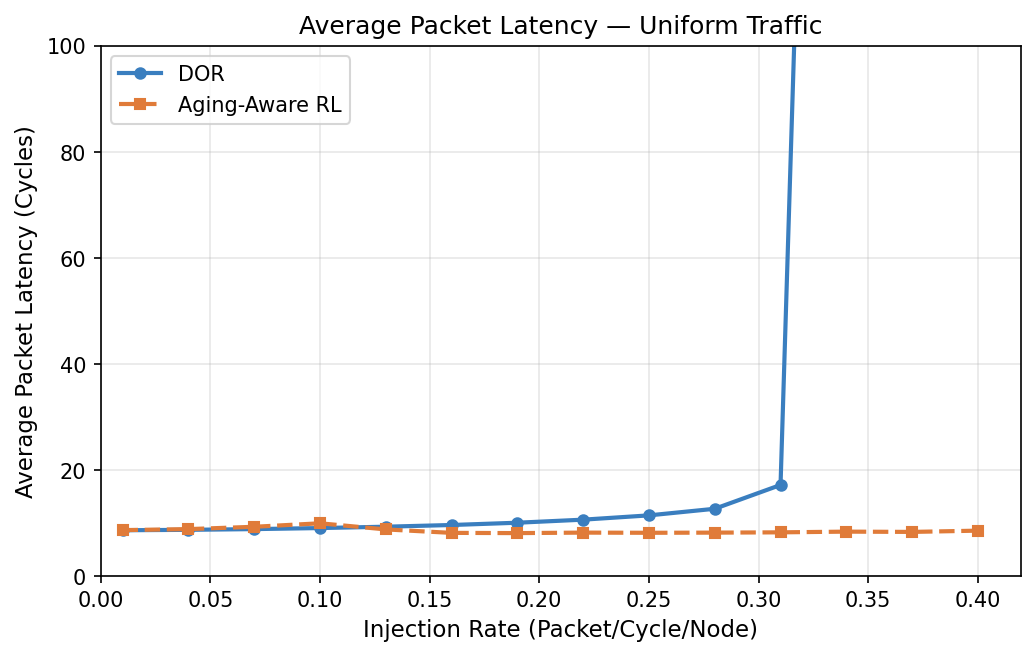
\includegraphics[width=0.8\linewidth]{body_chapters/chap_4/figs/latency_uniform.png}
    \caption{Average Packet Latency under Uniform Random Traffic.}
    \label{fig:uniform_latency}
  \end{subfigure}
  \vspace{1em}
  \begin{subfigure}{\linewidth}
    \centering
    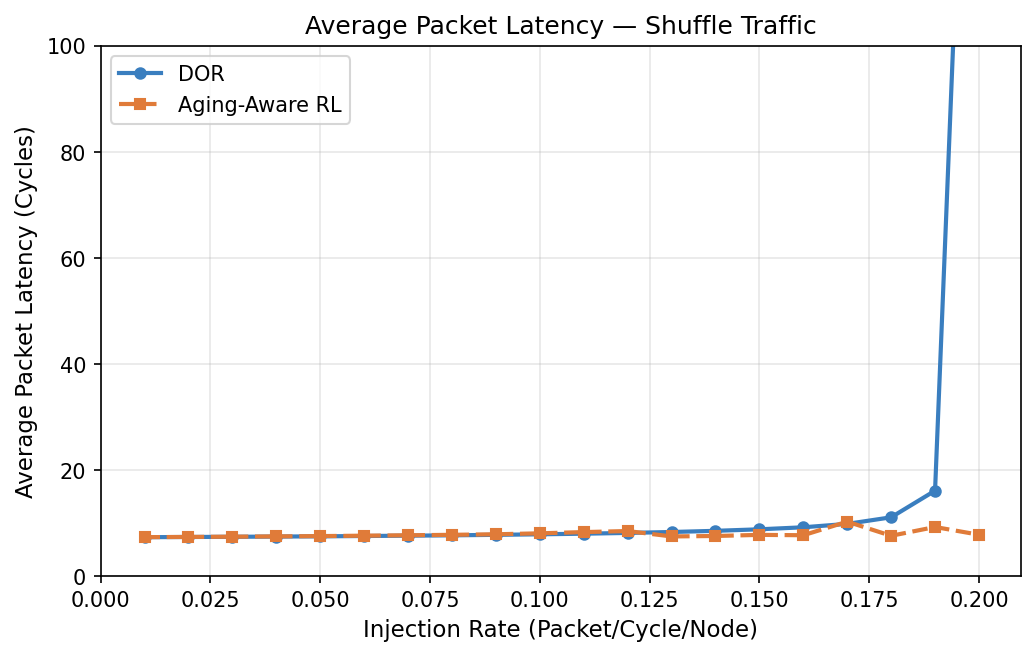
\includegraphics[width=0.8\linewidth]{body_chapters/chap_4/figs/latency_shuffle.png}
    \caption{Average Packet Latency under Shuffle Traffic.}
    \label{fig:shuffle_latency}
  \end{subfigure}
  \caption[Average Packet Latency (Uniform, Shuffle)]{Average Packet Latency vs. Injection Rate for RL-based Routing and DOR across Uniform Random and Shuffle traffic patterns.}
  \label{fig:latency_curves_2}
\end{figure}

\begin{figure}[ht]
  \centering
  \begin{subfigure}{\linewidth}
    \centering
    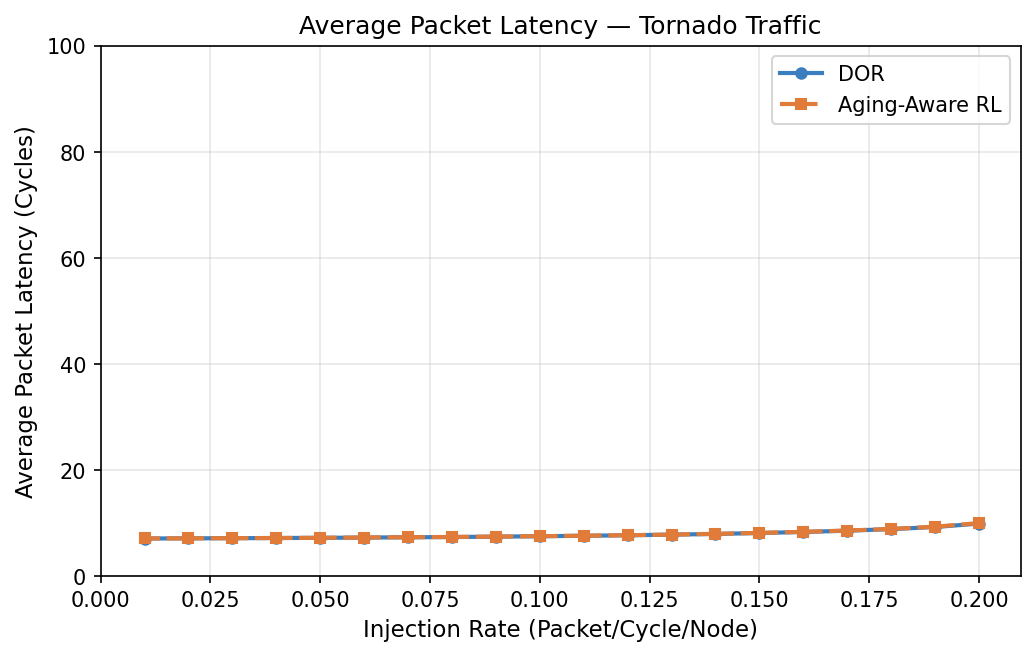
\includegraphics[width=0.8\linewidth]{body_chapters/chap_4/figs/latency_tornado.png}
    \caption{Average Packet Latency under Tornado Traffic.}
    \label{fig:tornado_latency}
  \end{subfigure}
  \vspace{1em}
  \begin{subfigure}{\linewidth}
    \centering
    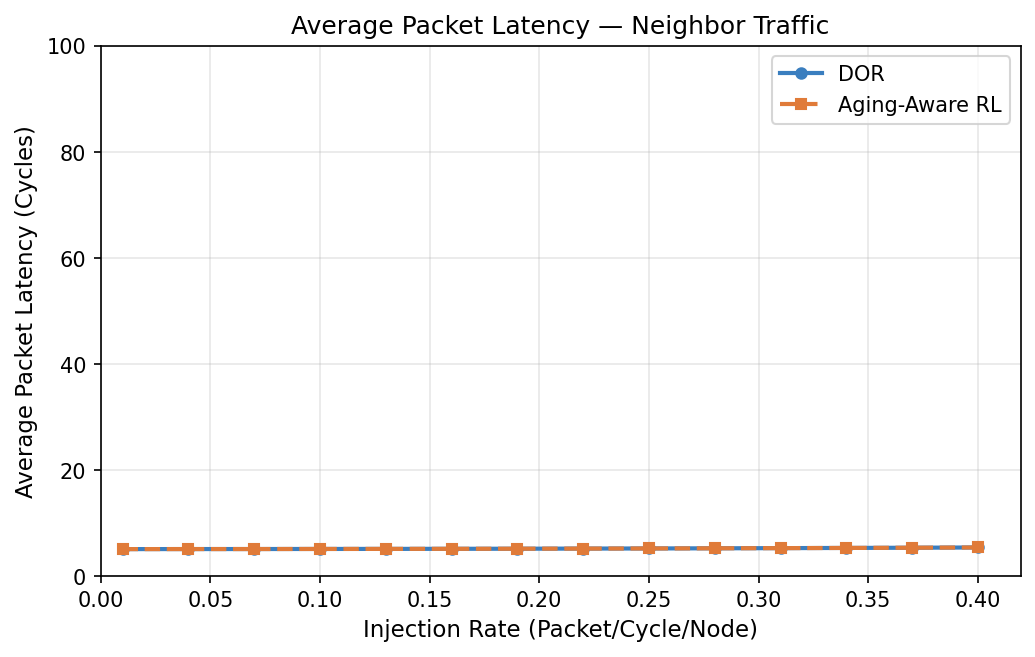
\includegraphics[width=0.8\linewidth]{body_chapters/chap_4/figs/latency_neighbor.png}
    \caption{Average Packet Latency under Neighbor Traffic.}
    \label{fig:neighbor_latency}
  \end{subfigure}
  \caption[Average Packet Latency (Tornado, Neighbor)]{Average Packet Latency vs. Injection Rate for RL-based Routing and DOR across Tornado and Neighbor traffic patterns.}
  \label{fig:latency_curves_3}
\end{figure}

Across all traffic patterns, the RL-based routing achieves latency comparable to or better than the DOR baseline. At low injection rates, both routing schemes exhibit nearly identical latency. This is expected, as the network is lightly loaded and there is limited contention, leaving little opportunity for adaptive routing to improve performance.

At higher injection rates, the benefits of RL-based routing become more apparent. As traffic increases, DOR begins to saturate due to its deterministic nature, which concentrates traffic along fixed paths and creates congestion hotspots. This results in a sharp increase in packet latency beyond the saturation point. In contrast, the RL-based routing distributes traffic more evenly across available paths, delaying the onset of congestion and maintaining lower latency under higher load conditions.

The most significant latency improvements are observed in structured traffic patterns such as bit reverse, bit rotation, shuffle, transpose, and uniform random. These patterns provide multiple routing options, allowing the RL agent to effectively balance load and avoid congested regions. In these cases, RL not only improves reliability but also enhances network performance.

For neighbor and tornado traffic, both routing schemes exhibit similar latency. This is expected, as these patterns constrain packets to a limited set of shortest paths, leaving little flexibility for adaptive routing to redistribute traffic. As a result, RL does not provide a noticeable performance advantage in these scenarios, but importantly, it does not degrade performance either.

% This is a reference to a label in another chapter. Appendix~\ref{chap:app1}. You can always refer to other labels from other chapters with the \textbf{\textbackslash ref} command. 

% It is good practice to follow the latex prefix guidelines for label names:
% \begin{itemize}
%     \item \textit{ch}:	chapter
%     \item \textit{sec}:	section
%     \item \textit{subsec}:	subsection
%     \item \textit{fig}:	figure
%     \item \textit{tab}:	table
%     \item \textit{eq}:	equation
%     \item \textit{lst}:	code listing
%     \item \textit{itm}:	enumerated list item
%     \item \textit{alg}:	algorithm
%     \item \textit{app}:	appendix subsection
% \end{itemize}



% \section{Summary}
% \lipsum[5]
% \section{Future Work}
% \lipsum[6]